\section{Tiefenanpassungen durch Farbbilder}

Aus allen zuvor beschriebenen Verfahren werden letztendlich Tiefeninformationen, in Form von geometrischen Primitiven oder Punkten im Raum gewonnen. Diese werden passend zur aktuellen Kameraposition als Tiefenbild gerendert und füllen den Z-Buffer für eine entsprechende Überdeckung der virtuellen Objekte. Auf Grund von Sensorungenauigkeiten oder größeren Auflösungen der Rekonstruktionsverfahren können dabei fehlerhafte Tiefeninformationen im Z-Buffer gelangen, die zu Fehlern bei der Bestimmung der Überdeckung führen können. Dieses Phänomen ist am Beispiel der Pointcloud Projektion aus Kapitel \ref{sec:pc-projection} in Abbildung \ref{fig:pc-noise} zu erkennen. \\

\begin{figure}[h]
  \centering
	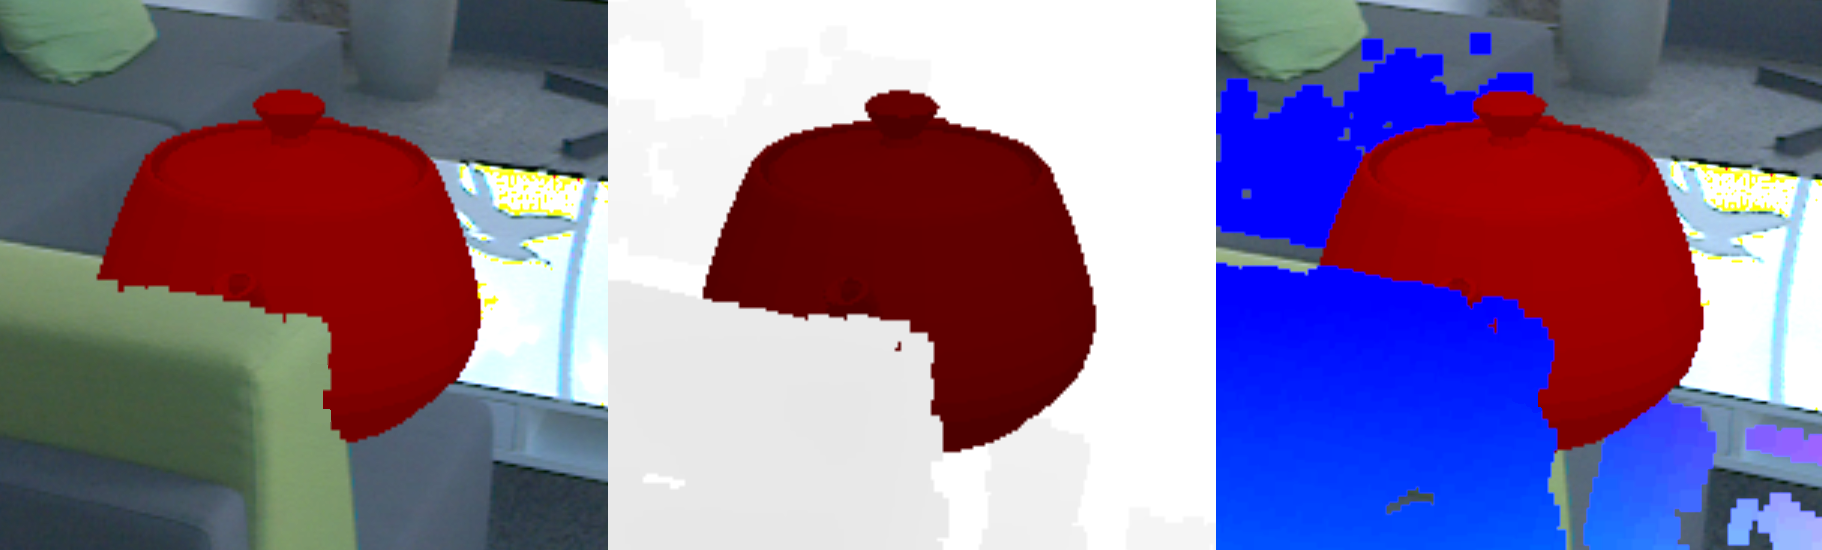
\includegraphics[width=1.0\textwidth]{content/images/methods/pc-noise.png} 
  \caption{Überdeckung mit einfacher Pointcloud Projektion. Links: Resultat der Überdeckung. Mitte: Darstellung des Tiefepuffers. Rechts: Darstellung der Pointcloud.}
  \label{fig:pc-noise}
\end{figure}

